\chapter{Practice: Collecting data in a computer}
\label{cha:sink-in-server}
\section*{Suggested read: Chapters~\ref{ATSensorNetwork} and~\ref{sunsetSensor}}

In this assignment we will use some Python libraries to receive the data transmitted by the sunset sensor in a computer instead of the Arduino.
You can use one of the university computers, a laptop or a RaspBerry.

Install the XBee Python libraries.

\url{http://pypi.python.org/pypi/XBee/2.0.0}

This code offers an implementation of the XBee serial communication API.

We re-use the processing board of the previous assignment (refer to Chapter~\ref{sunsetSensor}) and this time we will connect the XBee that receives the data to the computer using the USB cable.
Remember that in the last assignment it was connected to the Arduino.

\begin{lstlisting} [caption = {Simple code that reads the message that arrive to the XBee.}, language = Python, label = {code:simple-receiver}, numbers = left, escapeinside={@}{@}]

import serial
from xbee import ZigBee

print 'Printing data from remote XBee'

serial_port = serial.Serial('/dev/ttyUSB0', 9600)
zigbee = ZigBee(serial_port)

while True:
    try:
        print zigbee.wait_read_frame()
    except KeyboardInterrupt:
        break

serial_port.close()
\end{lstlisting}

You can see the results of running the program in Fig. \ref{fig:sink_in_server_screenshot_first_test}.

\begin{figure}[htbp]
  \centering
  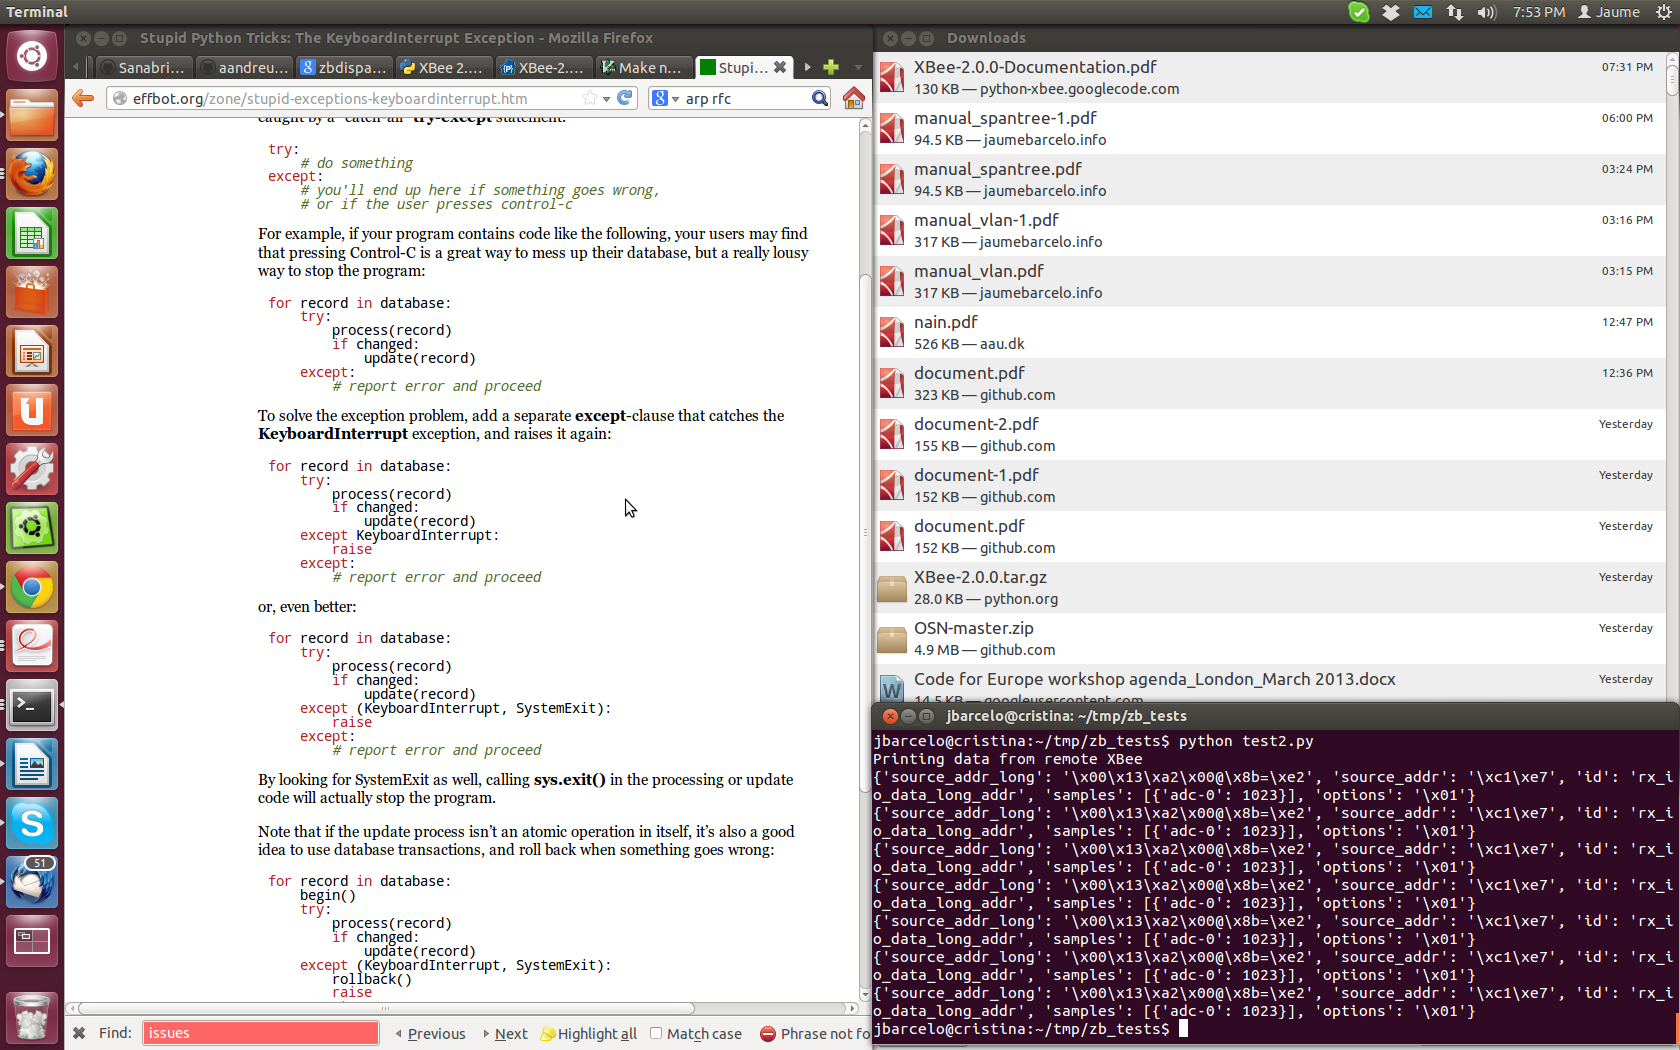
\includegraphics[width=0.9\linewidth]{figures/sink_in_server_screenshot_first_test.eps}
  \caption{A test run of a Python program to read the messages that arrive to the XBee.}
  \label{fig:sink_in_server_screenshot_first_test}
\end{figure}

If the processing of each incoming packet takes a long time, the processing must be made asynchronous so that newer packets can be also processed in parallel.
An example of long processing time can be uploading the data to the Internet.

We will define a (callback) function that is called whenever a packet is arrived.
See the Listing \ref{code:asynchronous-receiver} for example code.

\begin{lstlisting} [caption = {Simple code that asynchronously reads the message that arrive to the XBee.}, language = Python, label = {code:asynchronous-receiver}, numbers = left, escapeinside={@}{@}]

import serial
import time
from xbee import ZigBee

print 'Asynchronously printing data from remote XBee'

serial_port = serial.Serial('/dev/ttyUSB0', 9600)

def print_data(data):
    """
    This method is called whenever data is received.
    Its only argument is the data within the frame.
    """
    print data['samples']

zigbee = ZigBee(serial_port, callback = print_data)

while True:
    try:
        time.sleep(0.001)
    except KeyboardInterrupt:
        break

zigbee.halt();
serial_port.close()

\end{lstlisting}

You can change the configuration of your router from the coordinator. 
The code snippet in Listing \ref{code:sampling-rate}.

\begin{lstlisting} [caption = {This example remotely sets the configuration of the XBee, in particular the sample rate.}, language = Python, label = {code:sampling-rate}, numbers = left, escapeinside={@}{@}]

zigbee.send('remote_at',
          frame_id='A',
          dest_addr_long='\x00\x13\xa2\x00\x40\x8b\x3d\xe2',
          options='\x02',
          command='IR',
          parameter='\xF2')

\end{lstlisting}

Collaborate with other groups to create larger networks and explore what you can do with the data using Python programs (computing averages? sending an email upon a trigger event? dynamically adapting the sampling rate as a function of the measured vales?).

